\documentclass{article}
% PACKAGES %
\usepackage[english]{} % Sets the language
\usepackage[margin=2cm]{geometry} % Sets the margin size
\usepackage{fancyhdr} % Allows creation of headers
\usepackage{xcolor} % Allows the use of color in text
\usepackage{float} % Allows figures and tables to be floats
\usepackage{appendix}
\usepackage{amsmath} % Enhanced math package prepared by the American Mathematical Society
	\DeclareMathOperator{\sech}{sech} % Include sech
\usepackage{amssymb} % AMS symbols package
\usepackage{mathrsfs}% More math symbols
\usepackage{breqn} % Allows line breaking in math mode
\usepackage{cancel} % Allows math strikethroughs to show cancellations
\usepackage{bm} % Allows you to use \bm{} to make any symbol bold
\usepackage{bbold} % Allows more bold characters
\usepackage{verbatim} % Allows you to include code snippets
\usepackage{setspace} % Allows you to change the spacing between lines at different points in the document
\usepackage{parskip} % Allows you alter the spacing between paragraphs
\usepackage{multicol} % Allows text division into multiple columns
\usepackage{units} % Allows fractions to be expressed diagonally instead of vertically
\usepackage{booktabs,multirow,multirow} % Gives extra table functionality
\usepackage[final]{pdfpages} % Allows pdfs to be imported
\usepackage{hyperref} % Allows hyperlinks in the document
\usepackage{rotating} % Allows tables to be rotated
\usepackage{graphicx} % Enhanced package for including graphics/figures
	% Set path to figure image files
	\graphicspath{ {fig/} }
\usepackage{listings} % for including text files
	\lstset{basicstyle=\ttfamily\scriptsize,
        		  keywordstyle=\color{blue}\ttfamily,
        	  	  stringstyle=\color{red}\ttfamily,
          	  commentstyle=\color{gray}\ttfamily,
          	 }		
\newcommand{\tab}{\-\hspace{1cm}}

\newcommand{\p}{\partial}
\newcommand{\ppt}{\frac{\p}{\p t}}
\newcommand{\grad}{\vec{\nabla}}

\newcommand{\Xs}{\Sigma}
\newcommand{\xs}{\sigma}

\newcommand{\Oov}{\frac{1}{v}}

\newcommand{\pos}{\vec{r}}
\newcommand{\cur}{\vec{J}}
\newcommand{\Oh}{\hat{\Omega}}

\newcommand{\intfp}{\int_{4\pi}}
\newcommand{\intzi}{\int_0^{\infty}}


\newcommand{\rt}{(\pos,t)}
\newcommand{\rE}{(\pos,E)}
\newcommand{\rEO}{(\pos,E,\Oh)}
\newcommand{\rEt}{(\pos,E,t)}
\newcommand{\rEtprime}{(\pos,E',t)}
\newcommand{\rEOprime}{(\pos,E',\Oh')}
\newcommand{\rOt}{(\pos,\Oh,t)}
\newcommand{\rOtprime}{(\pos,\Oh',t)}
\newcommand{\rEOt}{(\pos,E,\Oh,t)}
\newcommand{\rEOtprime}{(\pos,E',\Oh',t)}
\newcommand{\EO}{(E,\Oh)}
\newcommand{\EOprime}{(E',\Oh')}
\newcommand{\EOt}{(E,\Oh,t)}



% Create a header w/ Name & Date
\pagestyle{fancy}
\rhead{\textbf{Mitch Negus} \; 12/1/2017}

\begin{document}
\thispagestyle{empty}

{\bf {\large {NE250 Homework {6} \hfill Mitch Negus\\
		\hspace*{\fill} 12/1/2017\\ }}}
		
		
		
%%%%%%%%%%%%%%%%%%%%%%%%%%%%%%%%%% PROBLEM 1 %%%%%%%%%%%%%%%%%%%%%%%%%%%%%%%%%%

\section*{Problem 1}

\subsection*{\textit{a.})}
Expected Value/Mean: 
\begin{align*}
\mu &= \int_{-\infty}^{\infty} x f(x) \, dx \\
	&= \int_0^a \frac{x}{a} \, dx  \\
	&= \frac{1}{2a}\left[x^2\right]_0^a
\end{align*}
$$\boxed{ \mu = \frac{a}{2} }$$
Variance:
\begin{align*}
\sigma^2	&= E[(X-\mu)^2] \\
			&= \int_{-\infty}^{\infty}(x-\mu)^2 f(x) \, dx \\
			&= \int_0^a \left(x-\frac{a}{2}\right)^2 \left(\frac{1}{a}\right) \, dx \\
			&= \int_0^a \left(x^2-ax+\frac{a^2}{4}\right) \left(\frac{1}{a}\right) \, dx \\
			&= \int_0^a \frac{x^2}{a} \, dx - \int_0^a x \, dx + \int_0^a \frac{a}{4} \, dx \\
			&= \left[ \frac{x^3}{3a} \right]_0^a - \left[ \frac{x^2}{2} \right]_0^a + \left[ \frac{ax}{4} \right]_0^a \\
			&= \frac{a^2}{3} - \frac{a^2}{2} + \frac{a^2}{4}
\end{align*}
$$\boxed{ \sigma^2 = \frac{a^2}{12} }$$
Cumulative Distribution Function:
\begin{align*}
F(x)	&= \int_{-\infty}^{x} f(x') dx' \\
		&= \int_0^x \frac{1}{a} \, dx' \\
		&= \frac{1}{a}\left[x'\right]_0^x \\
		&= \frac{x}{a}
\end{align*}
$$\boxed{ F(x) = \begin{cases}	0, & x < 0, x > a \\
								\frac{x}{a}, & 0 < x < a \end{cases}}$$
\subsection*{\textit{b.})}
Expected Value/Mean: 
\begin{align*}
\mu &= \int_{-\infty}^{\infty} x f(x) \, dx \\
	&= \int_0^{\infty} \lambda x e^{-\lambda x} \, dx  \\
(\text{let }u = \lambda x, du &= \lambda\,dx, dv = e^{-\lambda x}, v = -e^{-\lambda x}/\lambda)\\
	&= uv|_0^{\infty} - \int_0^{\infty}v \, du \\
	&= -x e^{-\lambda x}\bigg|_0^{\infty} - \int_0^{\infty} \frac{-\lambda e^{-\lambda x}}{\lambda} \, dx \\
	&= 0 + \left[ \frac{-e^{-\lambda x}}{\lambda} \right]_0^{\infty}
\end{align*}
$$\boxed{ \mu = \frac{1}{\lambda} }$$
Variance:
\begin{align*}
\sigma^2	&= E[(X-\mu)^2] \\
			&= E[X^2] - \mu^2 \\
			&= \int_0^{\infty}x^2 f(x) \, dx - \frac{1}{\lambda^2}  \\
			&= \int_0^{\infty}\lambda x^2 e^{-\lambda x} \, dx - \frac{1}{\lambda^2}  \\
(\text{let }u = \lambda x^2, du &= 2\lambda x\,dx, dv = e^{-\lambda x}, v = -e^{-\lambda x}/\lambda)\\
			&= uv|_0^{\infty} - \int_0^{\infty}v \, du - \frac{1}{\lambda^2} \\
			&= \left[ -x^2 e^{-\lambda x}) \right]_0^{\infty} + \int_0^{\infty} 2 x e^{-\lambda x} \, dx - \frac{1}{\lambda^2}\\
			&= 0 + 2 \int_0^{\infty} x e^{-\lambda x} \, dx - \frac{1}{\lambda^2}\\
			&= \frac{2}{\lambda^2} \left[ e^{-\lambda x}(-\lambda x-1) \right]_0^{\infty} - \frac{1}{\lambda^2}\\
			&= \frac{2}{\lambda^2} - \frac{1}{\lambda^2}
\end{align*}
$$\boxed{ \sigma^2 = \frac{1}{\lambda^2} }$$
Cumulative Distribution Function:
\begin{align*}
F(x)	&= \int_{-\infty}^{x} f(x') dx' \\
		&= \int_0^x \lambda e^{-\lambda x'} \, dx' \\
		&= \left[-e^{-\lambda x'}\right]_0^x \\
		&= \left[1 -e^{-\lambda x} \right]
\end{align*}
$$\boxed{ F(x) = 1 -e^{-\lambda x} }$$



%%%%%%%%%%%%%%%%%%%%%%%%%%%%%%%%%% PROBLEM 2 %%%%%%%%%%%%%%%%%%%%%%%%%%%%%%%%%%

\section*{Problem 2}

(See Jupyter notebook, attached)



%%%%%%%%%%%%%%%%%%%%%%%%%%%%%%%%%% PROBLEM 3 %%%%%%%%%%%%%%%%%%%%%%%%%%%%%%%%%%

\section*{Problem 3}
\subsection*{\textit{a.})}
\subsection*{\textit{b.})}
\subsection*{\textit{c.})}
\subsection*{\textit{d.})}
\subsection*{\textit{e.})}
\subsection*{\textit{f.})}
\subsection*{\textit{g.})}



%%%%%%%%%%%%%%%%%%%%%%%%%%%%%%%%%% PROBLEM 4 %%%%%%%%%%%%%%%%%%%%%%%%%%%%%%%%%%

\section*{Problem 4}





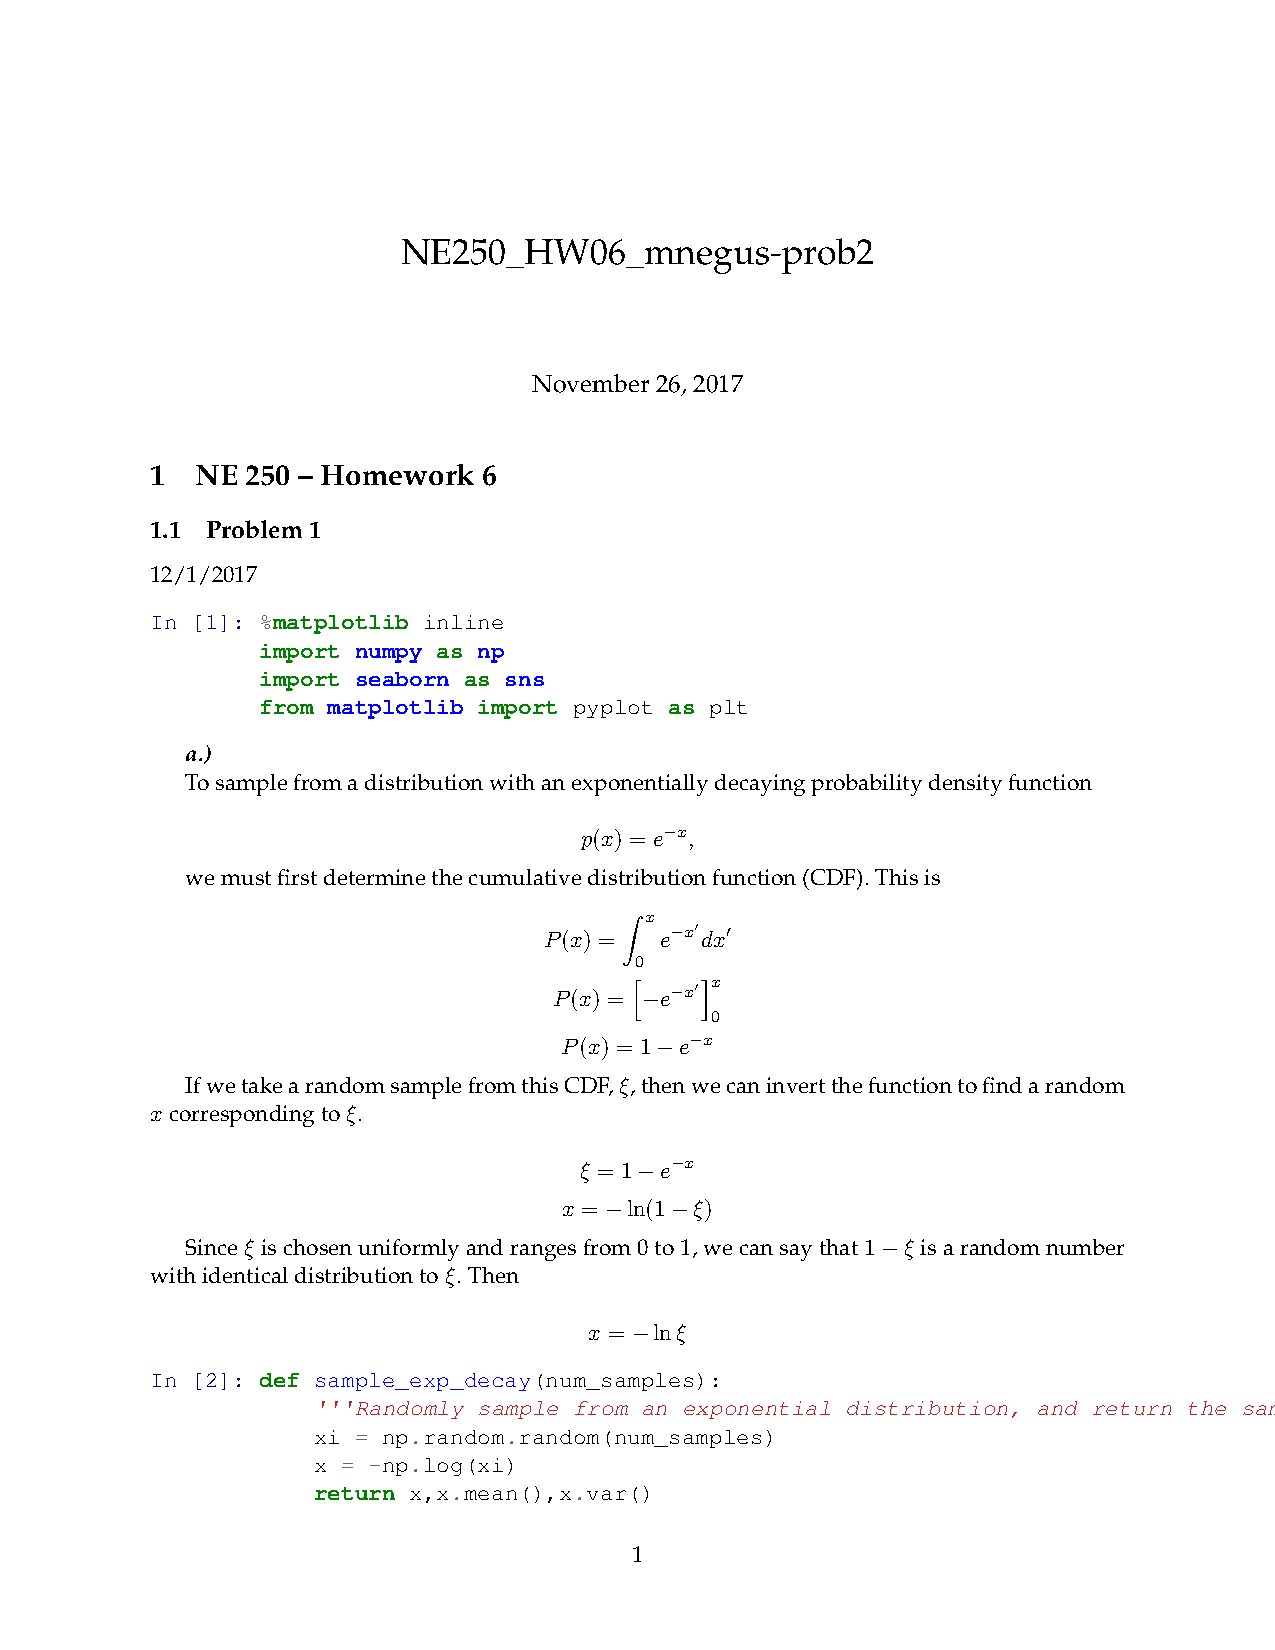
\includepdf[pages=-]{NE250_HW06_mnegus-prob2.pdf}
%\includepdf[pages=-]{NE250_HW05_mnegus-prob{...}.pdf}


\end{document}





 
